%%%%%%%%%%%%%%%%%%%%%%%%%%%%%%%%%%%%%%%%%%%%%%%%%%%%%%%%%%%%%%%%%%%%%%%%%%%%%%%%%%%%%%%%%%%%%%%%%%%%%%%%%%%%%%%%
%%%%%%%%%%%%%%%%%%%%%%%%%%%%%%%%%%%%%%%%%%%%%%%%%%%%%%%%%%%%%%%%%%%%%%%%%%%%%%%%%%%%%%%%%%%%%%%%%%%%%%%%%%%%%%%%
%%%%%                                          MAGNETISMUS                                             %%%%%%%%%
%%%%%%%%%%%%%%%%%%%%%%%%%%%%%%%%%%%%%%%%%%%%%%%%%%%%%%%%%%%%%%%%%%%%%%%%%%%%%%%%%%%%%%%%%%%%%%%%%%%%%%%%%%%%%%%%
%%%%%%%%%%%%%%%%%%%%%%%%%%%%%%%%%%%%%%%%%%%%%%%%%%%%%%%%%%%%%%%%%%%%%%%%%%%%%%%%%%%%%%%%%%%%%%%%%%%%%%%%%%%%%%%%
\skriptsection{Das Magnetische Feld}{5-1}

\skriptsubsection{Energie und Kraft im magnetischen Feld}{5-50}
\textbf{Energiedichte:}
$\boxed{w_m=\int_0^B{\vec{H}\cdot d\vec{B}}}$ (Allgemein)
$\qquad\boxed{w_m=\frac{1}{2}B\cdot H}$ (homog. Feld) $\qquad [w_m]=\frac{J}{m^3}$\\

\textbf{Energie:}
$\boxed{W_m = \frac{1}{2} L \cdot I^2=\frac{1}{2} N \cdot I \cdot
\Phi \; \text{ or } \; W_m=\frac{1}{2} \int_{V_{Lu}} \vec H \cdot
\vec B \cdot dV}$ (Allg.)
$\quad\boxed{W_m=w_m \cdot V=\frac{1}{2} B \cdot H \cdot V}$ (homog. Feld)\\ \\
\parbox{5cm}{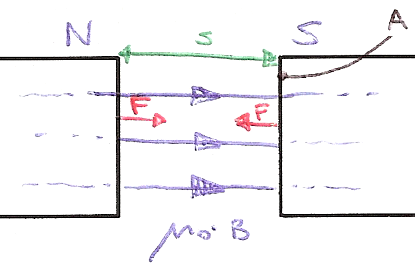
\includegraphics[width=4cm]{./bilder/m-kraft-mfeld.png}}
\parbox{13cm}{	
	Die Kraft auf Grenzflächen ist stets so gerichtet, dass sie die Induktivität
	zu vergrössern sucht. Das heisst immer vom ferromagnetischen Material zur
	nichtferromagnetischen Umgebung (z.B. Luft). Prinzip der virtuellen
	Verschiebung:\\
	\textbf{Kraft auf einen Anker:}
	$$\boxed{F = \left| \frac{\mathrm dW_m}{\mathrm ds} \right| = \frac{1}{2} I^2 \cdot 	
	\frac{\mathrm dL}{\mathrm ds} \qquad oder \qquad  F = \frac{1}{2} B_L \cdot H_L \cdot A_L}$$ 
	\\ 
	$$\boxed{ F= \frac{1}{2}\frac{B_L^2}{\mu_0}  A_L =  
				\frac{1}{2} \mu_0 \cdot H_L^2 \cdot A_L =  
				\frac{1}{2} \frac{\Phi^2}{\mu_0 A_L} =
				\frac{1}{2} \frac{\Phi \cdot B_L}{\mu_0}
			} \text{ (für } \mu_{rFe} \gg  \text{ 1)}$$}

\newpage
\subsection{Wichtigste Formeln}
	Magnetische Feldlinien verlaufen ausserhalb eines Magneten vom Nord- zum Südpol
	und sind immer geschlossen. Dabei zeigt die Kompassnadel immer in Richtung der 
	Feldlinien.\\
	\renewcommand{\arraystretch}{1.8}
	\begin{tabular}[c]{ | p{5cm} | p{8cm} | p{4cm} | }
		\hline
		\textbf{Name} 
		& \hspace{-6pt}\begin{tabular}[t]{p{3.8cm} | p{3.8cm}}
			\textbf{Allg.}
			& \textbf{Homogen}
			\\
		 \end{tabular} 
		& \textbf{Info}\\    
		\hline
	Permeabilität
		& $\mu_0 = 4 \pi \cdot 10^{-7} \frac{Vs}{Am} = 1.2566 \frac{\mu H}{m}$ \ \ \ $\mu = \mu_0 \cdot \mu_r$
		&$\frac{\mu H}{m}=\frac{Vs}{An}$\\
		\hline 
	3-Finger-Regel: (rechte Hand)
		& $F$ = Daumen, $v$ = Zeigefinger, $B$ = Mittelfinger
		& $Q > 0$ !!\\
		\hline
		\hline

	Ampèresches Gesetz
		&$F_A=\underbrace{\frac{\mu}{4\pi} \frac{ \cdot Q_1 \cdot v_1}{r^2}}_{B} \cdot 
			Q_2\cdot v_2$
		&\\
		\hline

	Lorentzkraft (bewegte Ladung)
		& \hspace{-6pt}\begin{tabular}[t]{p{3.8cm} | p{3.8cm}}
			$\vec{F} = Q (\vec{v} \times \vec{B})$
			& $|\vec{F}| = Q \cdot v \cdot B \cdot \sin\alpha$
			\\	
		\end{tabular} 	
		&$N$\\
	Kraft auf stromführenden Leiter
		 & \hspace{-6pt}\begin{tabular}[t]{p{3.8cm} | p{3.8cm}}
			$\vec{F}_L=I(\vec{l}\times \vec{B})$
			& $|\vec{F}_L| =  I \cdot l \cdot B \cdot \sin\alpha$
			\\
		 \end{tabular} 
		&\\
		\hline
	
	Magn. Flussdichte 
		& $B = H \cdot \mu = \frac{F}{Q \cdot v}  \text{, wobei } \vec{v} \perp \vec{B}$ 
		& $\frac{Vs}{m^2} = T$ (Tesla) \\
		\hline		

	Magnetische Feldstärke
		& \hspace{-6pt}\begin{tabular}[t]{p{3.8cm} | p{3.8cm}}
			$\vec{H} = \frac{ \vec{B}}{\mu }$
			& $H(s) \text{ aus } \Theta = \mathring{V}_m$
			\\
		 \end{tabular}  
		& $\frac{A}{m}$\\
		\hline

	Magnetische Spannung
		& \hspace{-6pt}\begin{tabular}[t]{p{3.8cm} | p{3.8cm}}
			$V_{m} = \int\limits \vec{H}(s) \cdot \vec{ds}$
			& $V_{m} = H \cdot s$
			\\
		 \end{tabular} 
		 & $A$ \\
	Magn. Umlaufspannung
		& \hspace{-6pt}\begin{tabular}[t]{p{3.8cm} | p{3.8cm}}
			$\mathring{V}_m = \oint\vec{H}(s) \cdot \vec{ds}$
			& $\mathring{V}_m = H \cdot \mathring{s}$
			\\
		 \end{tabular} 
		 & \\
		\hline
	Durchflutungssatz
		& $\boxed{\Theta = \mathring{V}_m}  = \int\limits_A \vec{J}
		\cdot \vec{dA} \vee \underbrace{\sum I_k}_{= N I} = \oint\vec{H}(s) \cdot \vec{ds}$
		& $A$\\
		\hline
		\hline

	Magnetischer Fluss
		& \hspace{-6pt}\begin{tabular}[t]{p{3.8cm} | p{3.8cm}}
			$\Phi = \int\limits_A \vec{B} \cdot d\vec{A}$
			& $\Phi = B \cdot A \cdot \cos(\gamma)$
			\\
		 \end{tabular} 
		& $Vs = Wb$ (Weber)\\
		\hline
	Maxwellsche-Gleichung
		& $\oint \vec{B} \cdot \vec{dA} = 0$ ($\sum \Phi \text{ durch Hülle} = 0$)
		&\\
		\hline

	``Ohmsches	Gesetz des Magn.``
		& $ V_m = R_m \cdot \Phi  \Leftrightarrow \Theta = R_m \cdot \Phi \text{ (ganzer 
			Kreis)} $
		& $A$\\
		\hline

	Magn. Widerstand
		& \hspace{-6pt}\begin{tabular}[t]{p{3.8cm} | p{3.8cm}}
			$R_m = \frac{V_m}{\Phi} = \frac{\Theta}{\Phi}$
			&  $R_m = \frac{l}{\mu A}$
			\\
		 \end{tabular}  
		& $\frac{A}{Wb}$ \\
		
	Magn. Leitwert (auch $G_m/A_L$)
		& \hspace{-6pt}\begin{tabular}[t]{p{3.8cm} | p{3.8cm}}
			$\Lambda = \frac{1}{R_m} = \frac{\Phi}{V_m}=\frac{\Phi}{\Theta}$
			& $\Lambda = \frac{\mu A}{l}$
			\\
		 \end{tabular} 
		& $\frac{Vs}{A} = H$ (Henry) \\
		\hline
	Verketteter Fluss
		& $\Psi = \sum \Phi $ (meist $\boxed{\Psi = N \cdot \Phi}$)
		& $[\Psi] = [\Phi] = Vs = Wb$\\
		\hline
	\textit{Kopplung}
		& \hspace{-6pt}\begin{tabular}[t]{p{3.8cm} | p{3.8cm}}
			\textbf{Allg.}
			& \textbf{Bei best. Kopplung}
			\\
		 \end{tabular} 
		&\\
		\hline
	Induktivität
		& \hspace{-6pt}\begin{tabular}[t]{p{3.8cm} | p{3.8cm}}
			$L = \frac{\Psi}{I}$
			& ideal: $L = \Lambda N^2 = \frac{N^2}{R_m} $
			\\
		 \end{tabular} 
		& $[L] = \frac{Vs}{A} = H$\\
		\hline
	innere Induktivität
		& \hspace{-6pt}\begin{tabular}[t]{p{3.8cm} | p{3.8cm}}
			$L_i = \frac{\mu \cdot l}{8 \cdot \pi}$
			&
			\\
		 \end{tabular} 
		& $[L] = \frac{Vs}{A} = H$\\
		\hline
	Gegeninduktivität
		& \hspace{-6pt}\begin{tabular}[t]{p{3.8cm} | p{3.8cm}}
			$M = M_{21} = M_{12}$
			& ideal: $M = \sqrt{L_1 L_2}$
			\\
		 \end{tabular} 
		& vorder Index = Wirkung,\\
		& \hspace{-6pt}\begin{tabular}[t]{p{3.8cm} | p{3.8cm}}
			$M_{21} = \frac{\Psi_{21}}{I_1}$ ($= \frac{N_2 \Phi_{21}}{I_1}$)
			& nicht ideal: $M < \sqrt{L_1 L_2}$
			\\
		 \end{tabular} 
		& hinterer = Ursache\\
		\hline
	Kopplungsfaktor
		& \hspace{-6pt}\begin{tabular}[t]{p{3.8cm} | p{3.8cm}}
			$k = \frac{M}{\sqrt{L_1 L_2}}$
			& ideal: $k = 1$
			\\
		 \end{tabular} 
		& $[-]$ \\
		\hline

	Streukoeffizient
		& \hspace{-6pt}\begin{tabular}[t]{p{3.8cm} | p{3.8cm}}
			$\sigma = 1 - k^2 = 1 -\frac{M^2}{L_1 L_2}$
			& ideal: $\sigma = 0$
			\\
		 \end{tabular} 
		& $[-]$\\
		\hline
		\hline
	Hall-Sonde
		&$U_H = \frac{I \cdot B}{e \cdot n_p \cdot h}$
		& $V$\\
		\hline
	Kreis-r in M-Feld abgelenkte Q
		& $r = \frac{m_Q \cdot v}{Q \cdot B}$
		&m, $ m_e = 9,11 \cdot 10^{-31} kg$ \\
		\hline
	Füllfaktor
		&$F=\frac{A_{Effektiv Fe}}{A_{Tot}}$
		& $[-]$ ($F \le 1$)\\
		\hline
	Luftspaltkenngr\"osse
		&$\alpha = \frac{l_{Fe} \cdot A_L}{l_L \cdot A_{Fe}} \approx \frac{l_{Fe}}{l_L}$ (f\"ur $A_L \approx A_{Fe}$)
		&  $[-]$\\
		\hline
	effektive Permeabilit\"at
		&$\mu_{r_{eff}} = \frac{\alpha \cdot \mu_{r_{Fe}}}{\alpha + \mu_{r_{Fe}}}$
		&  $[-]$\\
		\hline
	\end{tabular}
	\renewcommand{\arraystretch}{1}
\newpage

\subsection{Magn. Feldstärke}
	\begin{tabular}[c]{l l}
	Biot-Savart: (Str\"ome d\"unner Leiter)
	& (bewegte Punktladung)\\ 
		$\vec{H}$ (in Punkt P) $= \frac{I}{4\pi} \int \frac{\vec{dl} \times\vec{r(l)}}{r^3(l)}$
		&$\vec{H} = \frac{Q}{4\cdot \pi \cdot r^3} \cdot (\vec{v} \times \vec{r})$\\
		&\\

	Magnetfeld ausserhalb eines langen Leiters:
	&Magnetfeld innerhalb eines geraden, langen Leiters: \\
		$H(r) = \frac{I}{2 \cdot \pi \cdot r}$
		&$H(r) = \frac{I}{2 \pi r} \frac{A_{eingeschlossen}}{A_{total}} $\\
		& \\
	Magnetfeld der Zylinderspule:
	&Magnetfeld einer Toroidspule:\\
		$H(r) = \frac{N \cdot I}{l} \qquad l \gg d$
		& $H_{innen}(r) = \frac{N \cdot I}{2 \cdot \pi \cdot r} \qquad H_{aussen} = 0$
	\end{tabular}

\renewcommand{\arraystretch}{1}

\begin{tabular}{llll}
	\parbox{4cm}{
		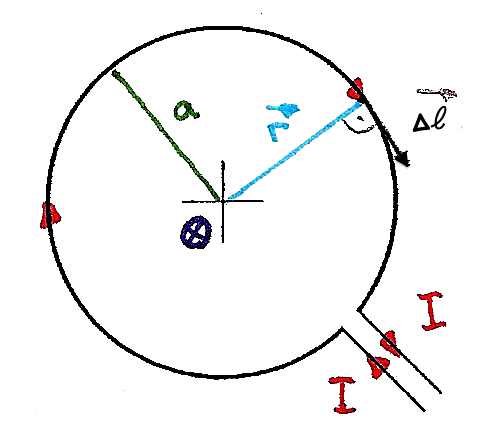
\includegraphics[width=2.7cm]{./bilder/biot1.png} \\
		$H =\frac{I}{D} = \frac{I}{2a}$}
	& \parbox{5cm}{
		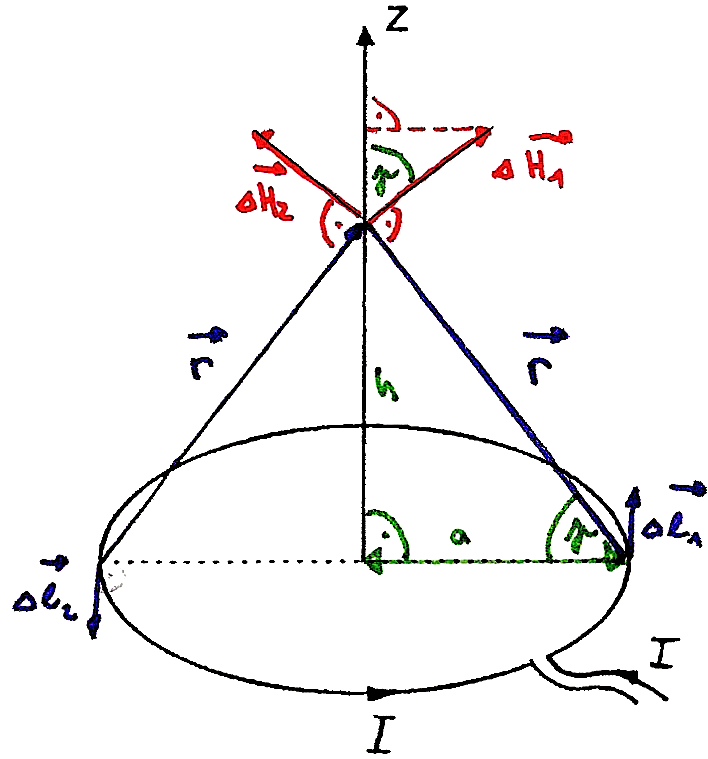
\includegraphics[width=2.7cm]{./bilder/biot2.png} \\
		$H=\frac{I}{2} \cdot \frac{a^2}{\sqrt{a^2+h^2}^3} = \frac{I}{2} \cdot 
			\frac{cos(\gamma)\cdot a}{2\vec{r}^2}$}
	& \parbox{4.5cm}{
		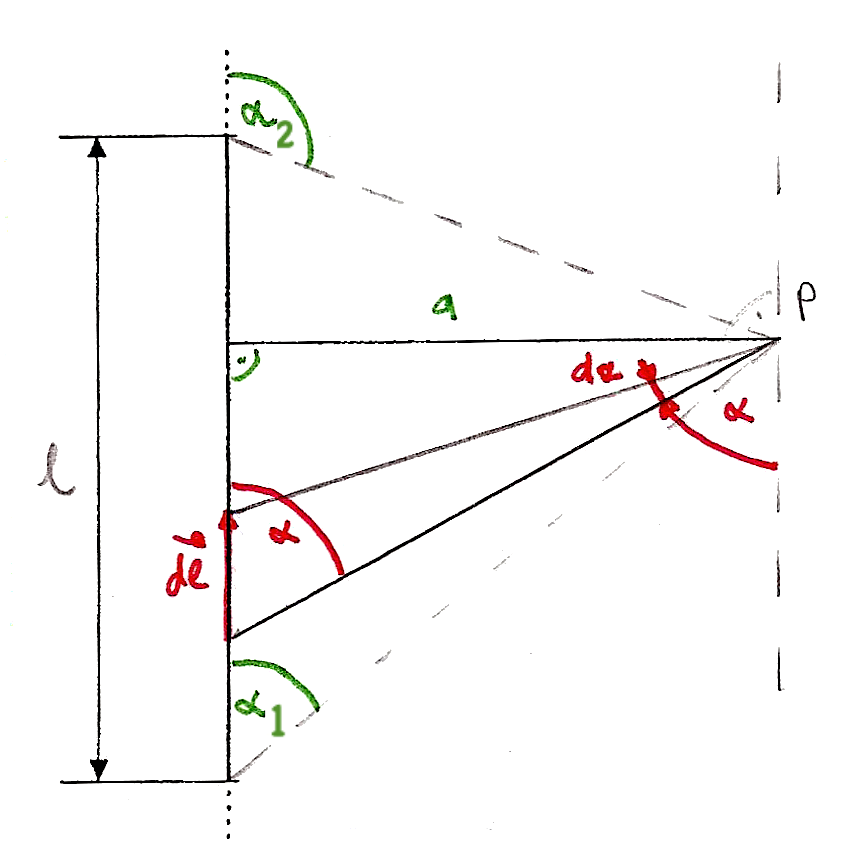
\includegraphics[width=3cm]{./bilder/biot3.png} \\
		$H=\frac{I}{4\pi a}(\cos \alpha_1- \cos \alpha_2)$}
	& \parbox{4.5cm}{
		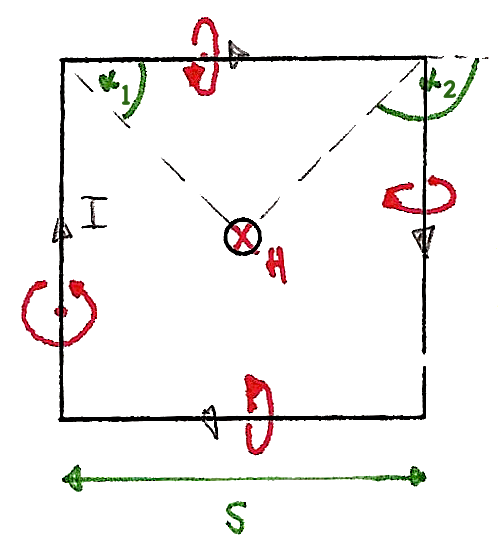
\includegraphics[width=2.7cm]{./bilder/biot4.png} \\
		$H= \frac{I \cdot 2 \sqrt{2}}{\pi \cdot s}$ }
\end{tabular}

\skriptsubsection{Induktivität}{5-23}
Induktivität hängt nicht vom Strom ab, sondern nur von der Geometrie der
Leiteranordnung, der Permeabilität und der umgebenden Materie.

\skriptsubsection{Gegeninduktivität, magnetische Kopplung}{5-26}
\begin{tabular}{ll}
\parbox{4.5cm}{
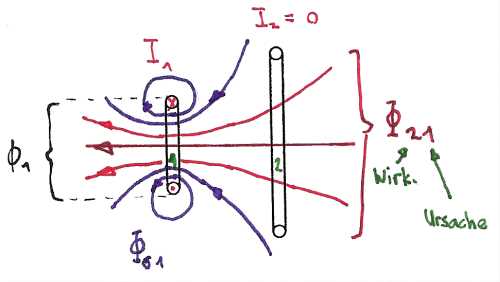
\includegraphics[width=4cm]{./bilder/gegeninduktivitaet.png}
}
& \parbox{14.5cm}{Die Gegeninduktivität beschreibt die Wirkung einer Spule auf
eine zweite, d.h. sie sind magnetisch gekoppelt.

Die magnetische Kopplung zweier Spulen hängt davon ab, ob und wie
gross der
Streufluss $\Phi_{\sigma}$, d.h. der Fluss, der ``verloren'' und nicht durch
die zweite Spule geht, ist. Je kleiner der Streufluss, desto idealer die
Kopplung.

$M=\sqrt{L_1L_2}\cdot k$ \ \ \ \ \ M = Reziprozität \ \ \ k = Kopplungsfaktor (= 1 falls ideal)}
\end{tabular}

\subsection{Zusammenstellung magnetischer Grössen für spezielle
Leiteranordnungen}
\begin{minipage}{14cm}
	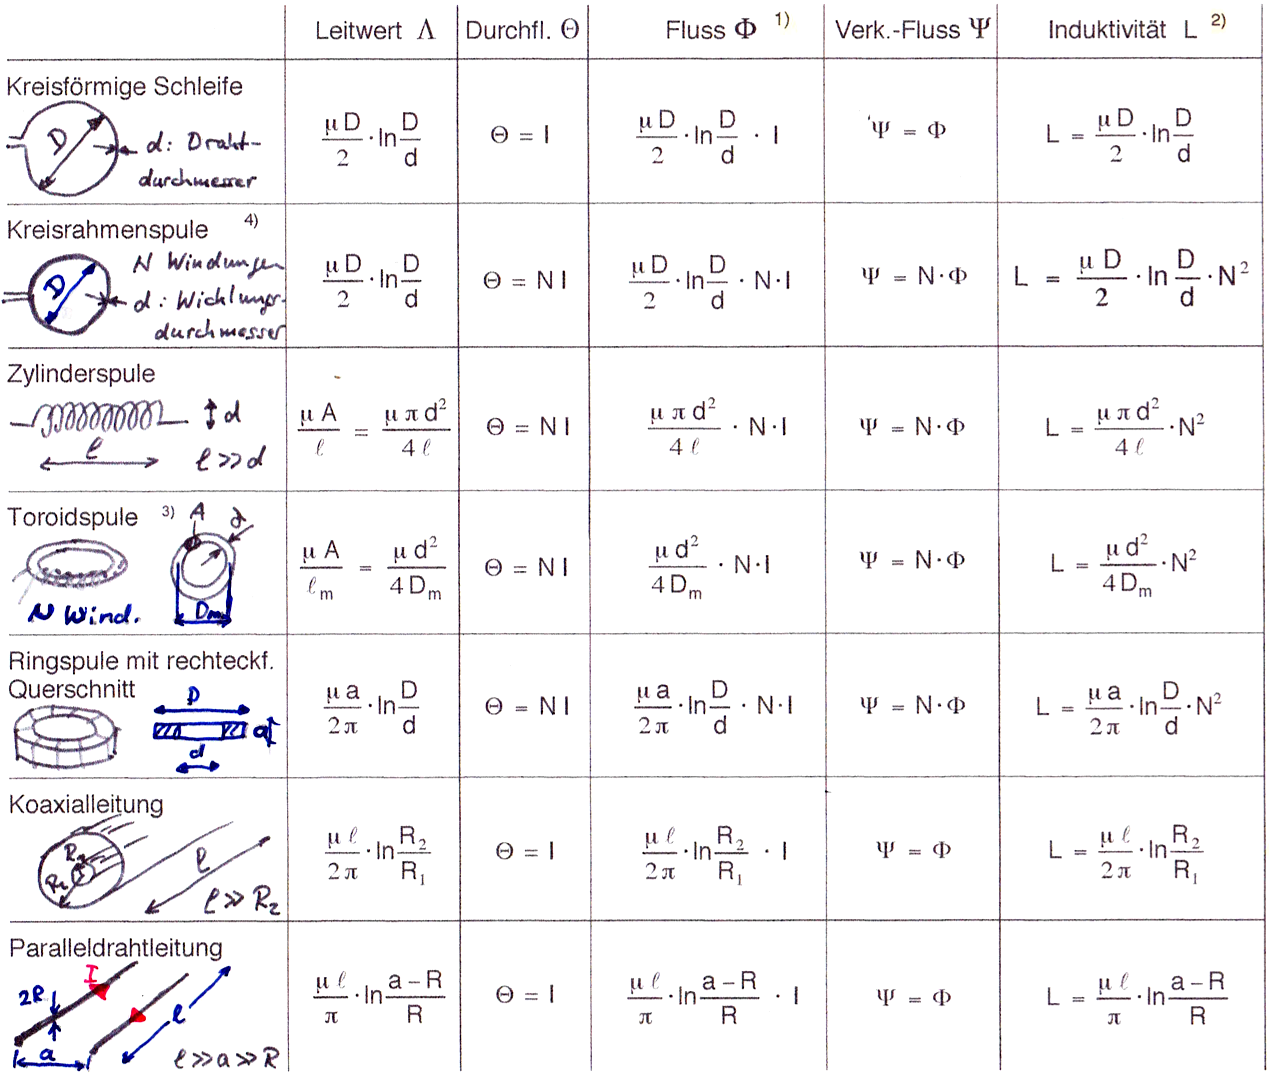
\includegraphics[width=12.5cm]{./bilder/magn_spez_leiteranordnungen.png} 
\end{minipage}
\begin{minipage}[ht]{5cm}
	\textbf{Bemerkungen:}\\
	$^{1)}$ ohne Fluss durch Leiter\\
	$^{2)}$ nur äussere Induktivität\\
	$^{3)}$ $A=\frac{\pi d^2}{4} \qquad l_m \approx \pi D_m$\\
	$^{4)}$ Wicklungs-$\varnothing$ d in radialer und axialer Richtung $d \ll D$\\
	
	\textbf{Allgemein} gilt:\\
	$\boxed{\Phi=\Lambda \cdot \Theta}$, $\Lambda=\frac{1}{R_m}$\\
	$\boxed{L=\frac{\Psi}{I}}$\\
	$L=\Lambda=\frac{1}{R_m}$, falls $N=1$\\
	$\boxed{L=\Lambda N^2=\frac{N^2}{R_m}}$, falls die $N$-Windungen unter sich ideal
	gekoppelt sind.
\end{minipage}

\skriptsubsection{Magnetisierung}{5-31}
\renewcommand{\arraystretch}{.25}
\begin{tabular}{|l|l|l|}
	\hline &&\\
	\parbox{5.5cm}{
	\textbf{Stoff (Eigenschaft)}\\
	\textit{Kennzeichen}} &
	
	\parbox{5.5cm}{
	Ohne äusseres Magnetfeld: Stoff magnetisch neutral, da\ldots } &
	
	\parbox{7cm}{
	Effekte beim Anlegen eines äusseren Magnetfeldes $H$
	} \\ &&\\ 
	\hline
	\hline &&\\
		
	\parbox{5.5cm}{
	\textbf{diamagnetisch}\\
	\textit{Felder bzw. Kreisströme der Elektronenbahnen eines Elementarteilchens
	kompensieren sich weitgehen} } &
	
	\parbox{5.5cm}{
	jedes einzelne Elemtarteilchen neutral
	} &
	
	\parbox{7cm}{
	Geringe Abschwächung des Feldes (Gegenfeld) infolge von Gegenkreisströmen:\\
	$\mu_r < 1$ } \\ &&\\
	\hline &&\\
	
	\parbox{5.5cm}{
	\textbf{paramagnetisch}\\
	\textit{Jedes Teilchen besitzt resultierenden Kreisstrom (resultierendes Feld)\\
	Teilchen = Elementarmagnet}
	} &
	
	\parbox{5.5cm}{
	Richtung der Elementartteilchen (Elementarmagnete) regellos	
	} &

	\parbox{7cm}{
	Verstärkung des Feldes durch Ausrichten der Elementarmangete in Richtung von $H$\\
	$\mu_r > 1$	} \\ &&\\
	\hline &&\\ 
	
	\parbox{5.5cm}{
	\textbf{ferromagnetisch}\\
	\textit{Bezirke aus vielen Elementarmagneten mit gleicher Magnetisierungsrichtung\\
	$\Rightarrow$ grössere Teilmagnete}} &
	
	\parbox{5.5cm}{
	Richtung der Bezirke regellos	
	} &
	
	\parbox{7cm}{
	- Ausrichten der Elementarmagnete\\
	- Vergrösserung der Bezirke mit gleicher Magnetisierungsrichtung wie H-Feld\\
	$\Rightarrow$ kräftige Verstärkung des Feldes\\
	$\mu_r >> 1 \qquad$ aber von H abhängig	
	} \\ &&\\
	\hline
\end{tabular}
\renewcommand{\arraystretch}{1}
\subsubsection{Ferromagnetische Stoffe}
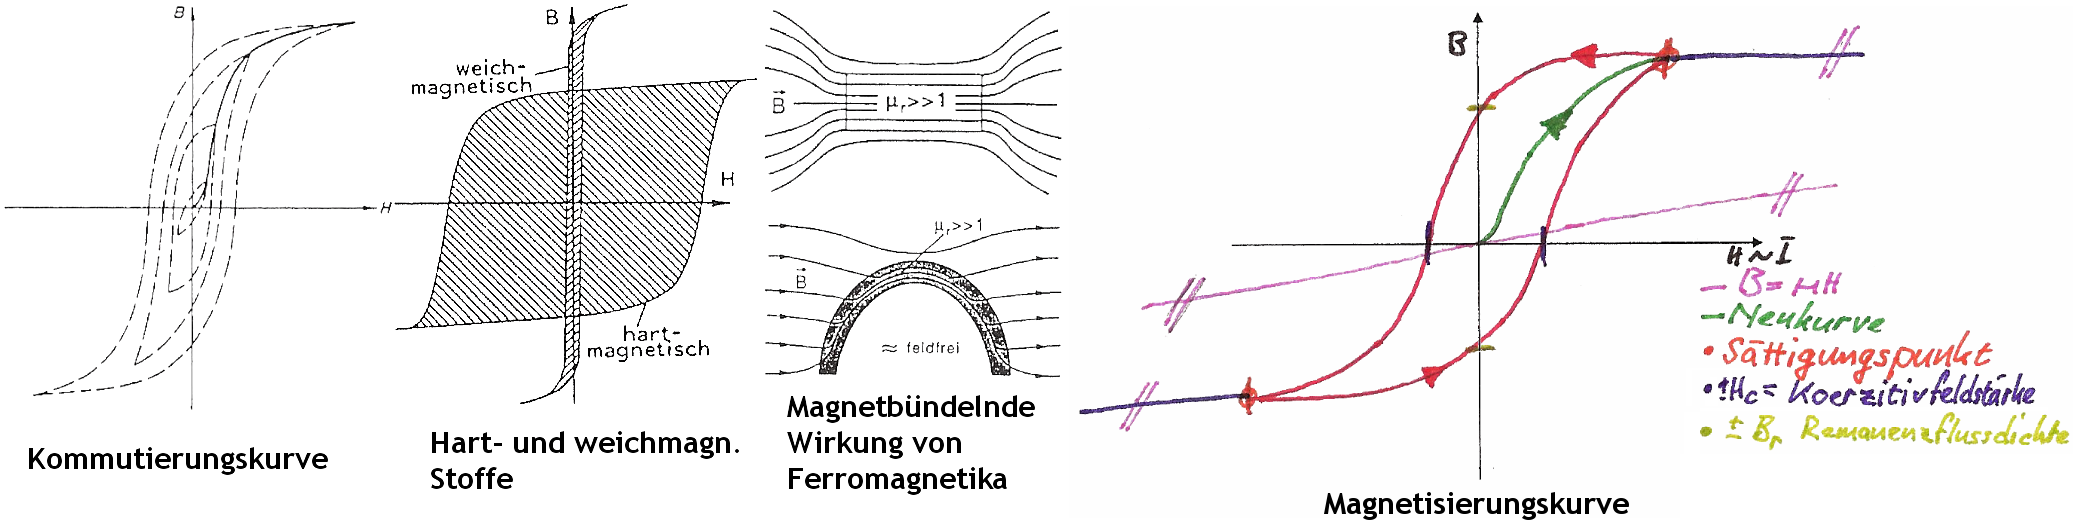
\includegraphics[width=16cm]{./bilder/magnetisierung.png}

\subsubsection{Brechung magnetischer Felder}
	Gleich wie bei elektrostischen Felder: $\frac{\tan(\alpha_1)}{\tan(\alpha_2)} = 
		\frac{\mu_{r1}}{\mu_{r2}} $ 


\subsection{Der magnetische Kreis}
\begin{minipage}{11cm}
	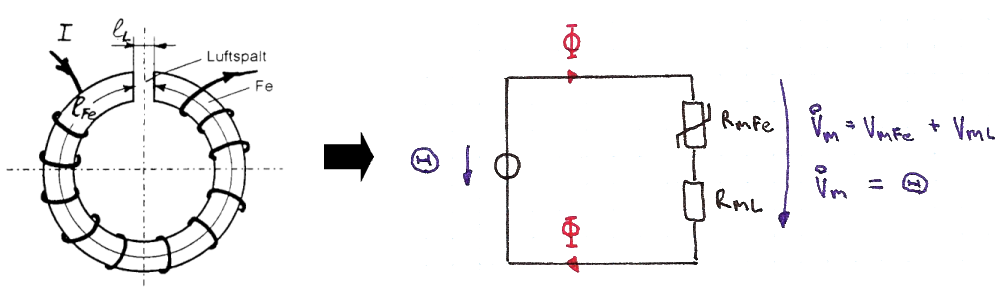
\includegraphics[width=11cm]{./bilder/magnetischerkreis1.png}
\end{minipage}
\hfill
\begin{minipage}{7cm}
\begin{tabbing}
xxxxxxx \= \kill  
$\mathring{V}_m$: \>magn. Umlaufspannung\\
$R_{mFe}$:\> magn. Wiederstand Eisenkern\\
$R_{mL}$:\> magn. Wiederstand Luft\\
$\Phi$:\> magn. Fluss\\
$ B \leftrightarrow H$:\> aus magn. Kurve\\
$\Theta = \mathring{V}_m = N \cdot I = \sum\limits_{i=1}^n H_i \cdot l_i$
\end{tabbing}
\end{minipage}

\subsubsection{Von der Durchflutung $\Theta$ ausgehende Berechnung}
\begin{minipage}{11cm}
	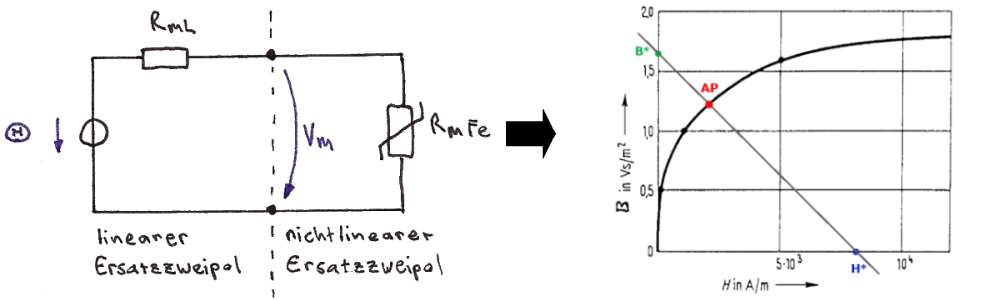
\includegraphics[width=11cm]{./bilder/magnetischerkreis2.png}
\end{minipage}
\hfill
\begin{minipage}{7cm}
\begin{tabbing}
xxx \= \kill  
1. \> magn. Kreis in linearen und nichtlinearen\\
   \> Teil aufteilen\\
2. \> Leerlaufspannung $V_{mLeerlauf}$ und\\
   \> Kurzschlussfluss $\Phi_k$ bestimmen\\
3. \> $H^*$ und $B^*$ bestimmen\\
4. \> $H^*$ und $B^*$ einzeichnen und\\
   \> Arbeitspunkt $AP$ bestimmen\\
5. \> $H$ und $B$ im AP herauslesen
\end{tabbing}
\end{minipage}
$$V_{mLeerlauf}=\Theta \qquad \Phi_k=\frac{\Theta}{R_{mL}}=\frac{\Theta \cdot
\mu_0 \cdot A_L }{l_L} \qquad H^*=\frac{\Theta}{l_{Fe}} (B = 0) \qquad B^*=\frac{\Phi_k}{A_{Fe}}=\frac{\Theta \cdot
\mu_0 \cdot A_L }{l_L A_{Fe}}=\overbrace{\frac{\mu_0 \cdot
\Theta}{l_L}}^{A_L=A_{Fe}}(H=0)$$


\subsection{Der magnetische Kreis mit Permanentmagnet}
\begin{minipage}{8cm}
	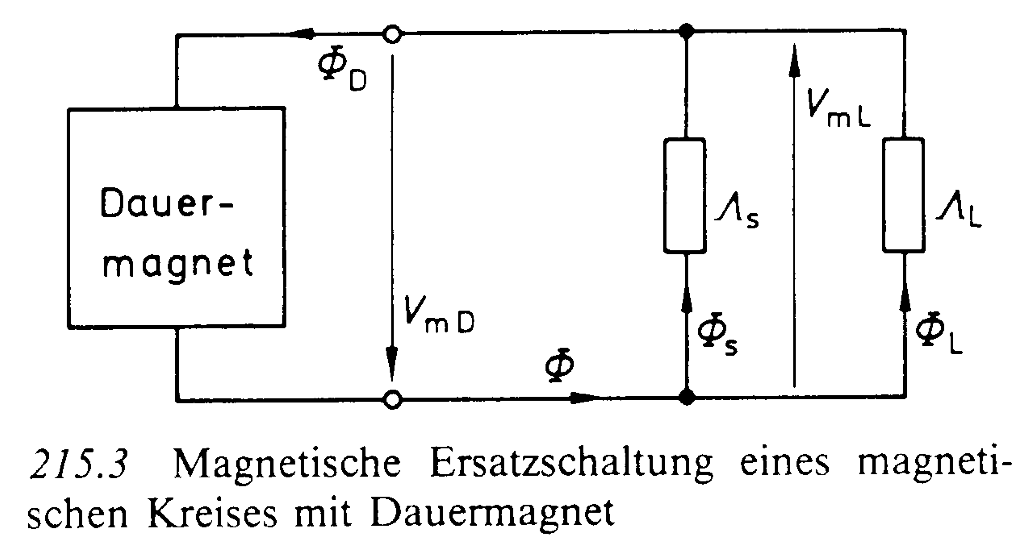
\includegraphics[width=8cm]{./bilder/DauerMag_Schaltung.png} \\
	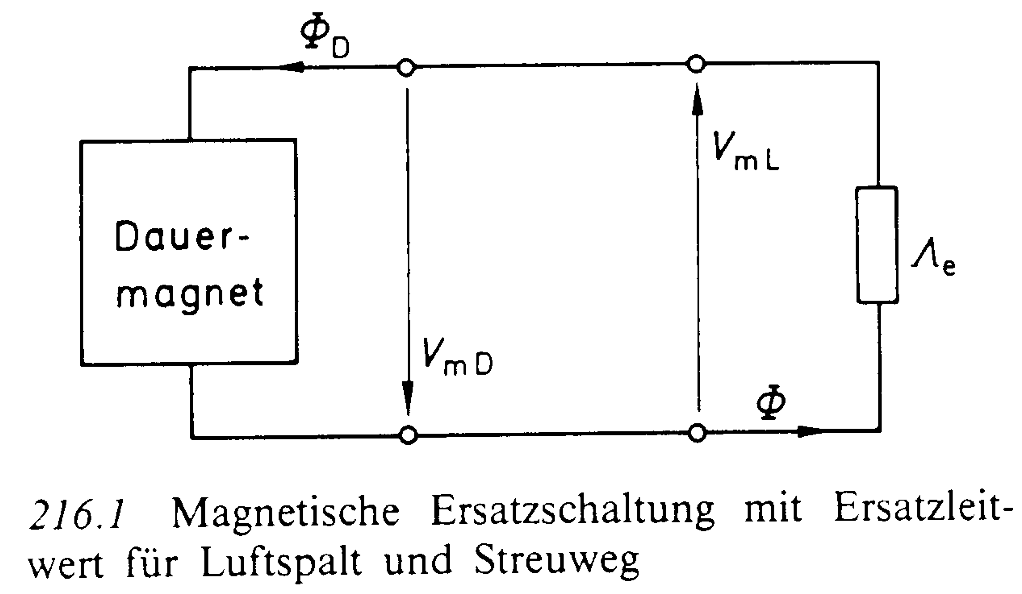
\includegraphics[width=8cm]{./bilder/DauerMag_Ersatzschaltung.png}
\end{minipage}
\hfill
\begin{minipage}{5cm}
	$V_{mD} = -V_{mL}$ \\
	
	$\Phi = \Phi_D = \frac{1}{s} \cdot \Phi_L = \Lambda_e \cdot V_{mL}$ \\
	
	$\Lambda_e = \frac{1}{s} \cdot \frac{\Phi_L}{V_{mL}} = \frac{1}{s} \cdot \Lambda_L = \frac{\mu_0 \cdot A_L}{s \cdot l_L}$ \\
	
	$H_L \cdot l_L = - H_D \cdot l_D$ \\
	
	$B_L = \mu_0 \cdot H_L = -\frac{\mu_0 \cdot H_D \cdot l_D}{l_L}$ \\
	
	$B_L = \frac{s \cdot A_D \cdot B_D}{A_L}$ \\
	
	$\rightarrow$ $\boxed{A_D = \frac{B_L \cdot A_L}{s \cdot B_D}}$ \\
	
	$\rightarrow$ $\boxed{l_D = \frac{H_L \cdot l_L}{H_D}}$	
	
\end{minipage}
\hfill
\begin{minipage}{5cm}
	$\Phi_D$ : Fluss des Dauermagneten \\
	
	$V_{mD}$ : Mag. Spannung Dauermagnet \\
	
	$V_{mL}$ : Mag. Spannung Luftspalt \\
	
	$\Lambda_s$ : Mag. Leitwert Streuung \\
	
	$\Lambda_L$ : Mag. Leitwert Luftspalt \\
	
	$\Lambda_e$ : Mag. Ersatzleitwert \\
	
	$s$ : Streufaktor \\
	
	$B_D$ : $B_{opt}$ \\
	
	$H_D$ : $H_{opt}$ \\
	
	$A_D$ : optimale Fl\"ache des Dauermagneten \\
	
	$l_D$ : optimale L\"ange des Dauermagneten
		
\end{minipage}

\begin{minipage}{8cm}
	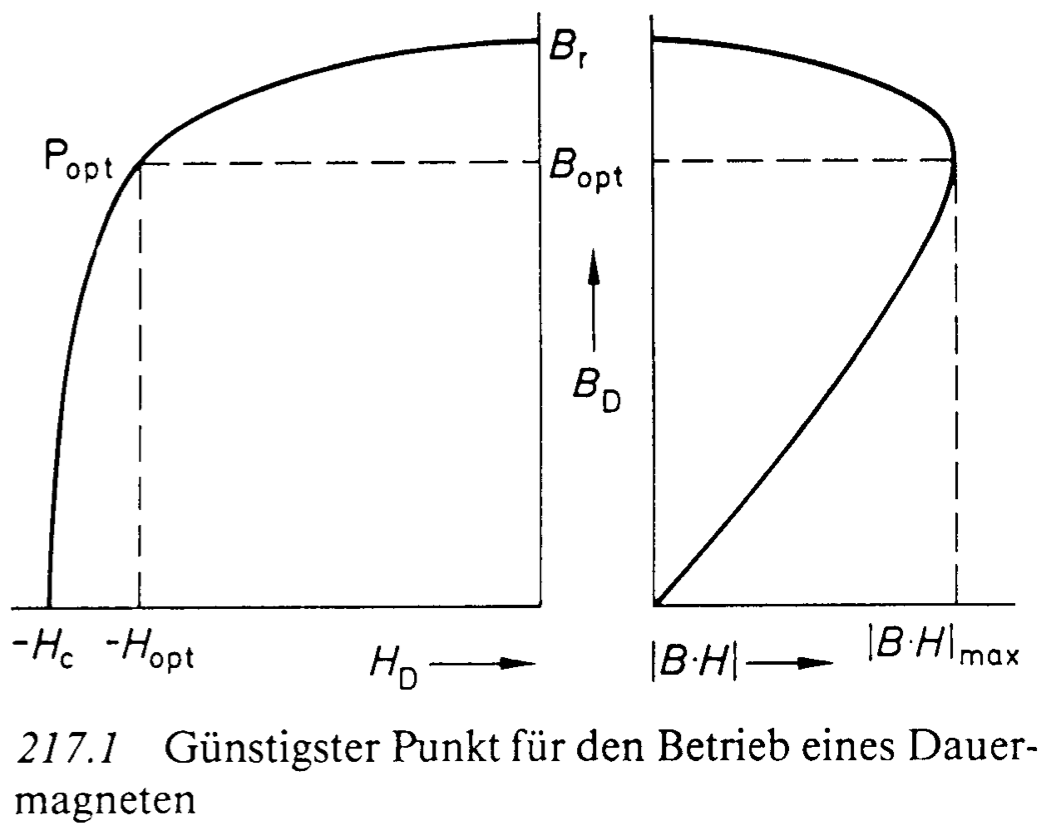
\includegraphics[width=8cm]{./bilder/BestArbeitspunktDauermagnet.png} 
\end{minipage}	
\hfill
\begin{minipage}{8cm}
	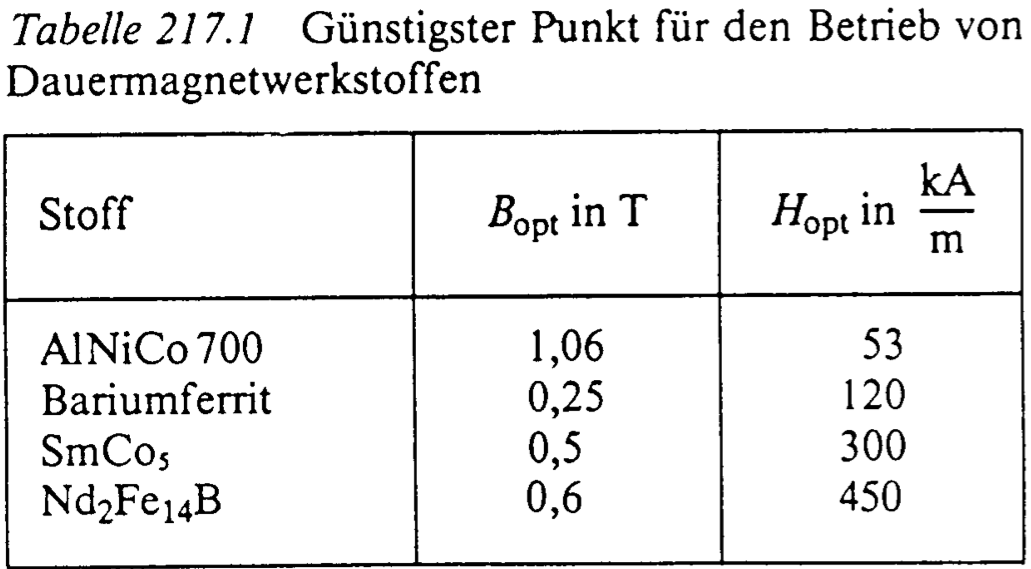
\includegraphics[width=8cm]{./bilder/BestArbeitspunktWerkstoff.png} 
\end{minipage}	


\newpage




